%%% Local Variables:
%%% mode: latex
%%% TeX-master: t
%%% End:
% --------------------------------------------------------------
% This is all preamble stuff that you don't have to worry about.
% Head down to where it says "Start here"
% --------------------------------------------------------------

\documentclass[12pt]{article}

\usepackage[margin=1in]{geometry}
\usepackage{amsmath,amsthm,amssymb}
\usepackage{graphicx}

\newcommand{\N}{\mathbb{N}}
\newcommand{\Z}{\mathbb{Z}}

\newenvironment{theorem}[2][Theorem]{\begin{trivlist}
\item[\hskip \labelsep {\bfseries #1}\hskip \labelsep {\bfseries #2.}]}{\end{trivlist}}
\newenvironment{lemma}[2][Lemma]{\begin{trivlist}
\item[\hskip \labelsep {\bfseries #1}\hskip \labelsep {\bfseries #2.}]}{\end{trivlist}}
\newenvironment{exercise}[2][Exercise]{\begin{trivlist}
\item[\hskip \labelsep {\bfseries #1}\hskip \labelsep {\bfseries #2.}]}{\end{trivlist}}
\newenvironment{reflection}[2][Reflection]{\begin{trivlist}
\item[\hskip \labelsep {\bfseries #1}\hskip \labelsep {\bfseries #2.}]}{\end{trivlist}}
\newenvironment{proposition}[2][Proposition]{\begin{trivlist}
\item[\hskip \labelsep {\bfseries #1}\hskip \labelsep {\bfseries #2.}]}{\end{trivlist}}
\newenvironment{corollary}[2][Corollary]{\begin{trivlist}
\item[\hskip \labelsep {\bfseries #1}\hskip \labelsep {\bfseries #2.}]}{\end{trivlist}}

\begin{document}

% --------------------------------------------------------------
%                         Start here
% --------------------------------------------------------------

%\renewcommand{\qedsymbol}{\filledbox}

\title{CS5214 Design of Optimizing Compilers }%replace X with the appropriate number
\author{Professor Weng-Fai Wong\\ %replace with your name
Assignment Two} %if necessary, replace with your course title

\maketitle

\abstract{This is the answer presented by Pan An. My student number is
  A0134556A. After tryin all the cool tools in Python, GNUPlot, and
  some books and papers, I finally figured out that this assignment is
not about programming. Alright so I'm just gonna present some results
that are partially calculated with my hand. Some of the math greatly
damaged my brain(kidding). Also I wanted to put a lot of references
but it seems that time is not enough for that. The folder contains
some of the rough calculation results performed by Python and some
other tools.}
% --------------------------------------------------------------
%     You don't have to mess with anything below this line.
% --------------------------------------------------------------
\section{The Lengauer‐Tarjan algorithm}

For the first question I simply assumn that in this diagram it does
not have very terrible effect by counting the {\bf start} and {\bf
  stop} nodes into the algorithm.

\subsection{Depth First Search}
I simply used {\bf networkx} in Python to do some of the graph
operation for me. The depth first search tree is stored in a picture
in {\bf img folder}.

After performing DFS on the tree, the DFT numbering is listed below in
the form of ($n_{DFT}$, Node). Node with number 0 and 100 are the
start and stop node.

\begin{verbatim}
(1, 0)
(2, 1)
(3, 2)
(4, 8)
(5, 31)
(6, 4)
(7, 5)
(8, 6)
(9, 7)
(10, 9)
(11, 10)
(12, 11)
(13, 12)
(14, 13)
(15, 14)
(16, 15)
(17, 16)
(18, 33)
(19, 18)
(20, 34)
(21, 21)
(22, 100)
(23, 3)
(24, 17)
(25, 19)
\end{verbatim}
Noticing that there could be multiple answers to DFS tree numbering, I
am using this one as the answer for the next couple questions.

\subsection{Dominators}
Most of the time semi-dominators of nodes in a graph is the immediate
dominator. To make it possible for people to compare, here is the result
for the immediate dominators of te graph(node: immediate dominator):
\begin{verbatim}
 0: 0,
 1: 0,
 2: 1,
 3: 31,
 4: 3,
 5: 4,
 6: 4,
 7: 3,
 8: 1,
 9: 8,
 10: 9,
 11: 10,
 12: 10,
 13: 12,
 14: 13,
 15: 14,
 16: 15,
 17: 33,
 18: 16,
 19: 34,
 21: 18,
 31: 1,
 33: 16,
 34: 18,
 100: 21
\end{verbatim}

And the semi-dominators I have computed is listed(node: semi-dominator):

$$ (0: 0), (1: 0), (3: 31), (4: 3), (5: 4), (6: 4), (7: 3), (8, 2)$$
$$ (9, 8), (10, 9), (11, 10), (12, 10), (13, 12), (14, 13), (15, 14)$$
$$ (16, 15), (17, 33), (18, 16), (19, 34), (21, 18), (31, 1), (33,
16), (100, 21)$$

\subsection{Control Dependency}


\subsection{Strongly Connected Componants}
A directed graph is called strongly connected if there is a path in
each direction between each pair of vertices of the graph.

Strongly connected graphs are(all edges amongs these nodes included):
\begin{itemize}
\item Nodes with self loop: 9, 13, 15, 19
\item Graph composed with node 16 and 33
\item Graph composed with node 3, 4, 6, 7
\item Graph composed with node 3, 4, 6, 7, 5
\item Graph composed with node 9, 10, 11
\end{itemize}

\subsection{Question 7}
Dominant frontier: 2, 16 and 18.

Block 33 should be inserted with the function.

\section{ Dataflow analysis}

The algorithm can be considered finding the node which  post-dominates
all node with the $USE(n)>0$. Also the node should be the 'first
one'.

Consider the following graph:
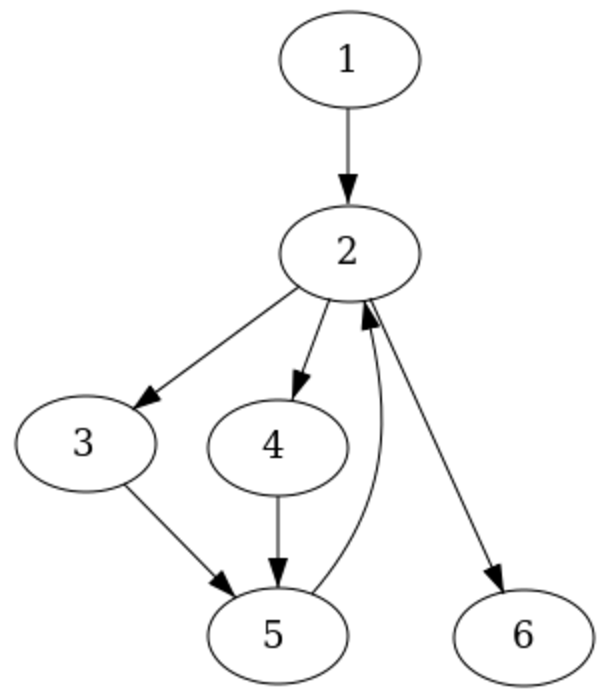
\includegraphics[scale=0.5]{pic1.png}

The algorithm is described below, it will return one single node that
satisfies the need:
\begin{itemize}
\item Initiate set $S_{u}, N_{p}$ as two empty sets;
\item DFS the graph, at the same time calculate $USE(n)$ for each
  node, and put all nodes with $USE(n)>0$ in to $S_{u}$;
\item Traverse the graph and calculate the the set of nodes each node post dominates(Lengauer
  and Tarjan’s Algorithm). Post dominating set of node $i$ is noted as
  $Dom_{i}$. If $S_{u} \subseteq Dom_{i}$, put node $i$ into $N_{p}$;
\item For node $i$ in $N_{p}$ after the traversal, if $N_{p} \cap
  Dom_{i}$ is empty, return the node and terminate the process.
\item Return the stop node(or none value found).
\end{itemize}

We assumn that in the graph node {\bf 2 and 4} are with a postive
$USE(n)$ value(variable is used). The algorithm will first traverse
the graph and find the variable usage, and after this process:
$$S_{u} = \{2, 4\}$$

After this the algorithm does another traversal. finding the nodes
that post dominates both 2 and 4. After this traversal:
$$N_{p} = \{6\}$$

And since this 6 is the only reason that post dominates both 2 and 4,
the algorithm returns node 6.

But when CFG is very large. The program will enumerate $N_{p}$ again
to find the first node that satisfies all the condition.
\end{document}
